\documentclass[12pt]{article}
\usepackage[margin=1in]{geometry}
\geometry{letterpaper}                  
\usepackage{graphicx}
\usepackage[hyphens]{url}
\usepackage{fancyhdr}
%\pagestyle{fancy}
\usepackage{fixltx2e}
\usepackage{amsmath,amsfonts,amsthm,amssymb}
\usepackage{graphicx}
\usepackage{algorithm}
\usepackage{algorithmic}
\usepackage{url}
\usepackage[normalem]{ulem}
%\usepackage[pdftex]{color}
\usepackage{varioref}
\usepackage{mathrsfs}
\usepackage{amsmath}
\labelformat{equation}{\textup{(#1)}}
\usepackage[sort&compress,colon,square,numbers]{natbib}
%\usepackage{cite}


\usepackage{color}
\newcommand{\todo}[1]{{\color{red}{\it TODO: #1}}}

\DeclareMathOperator*{\argmin}{arg\,min}


\begin{document}

\begin{center}\Large \bf EN.580.694: Statistical Connectomics \\ Final Project Report \end{center}
\begin{center} Michael Norris $\cdot$  \today \end{center}
\bigskip


\subsection*{Using a Random Dot Product Model to Approximate the C. Elegans Connectome}
$\\ \\$
\centerline{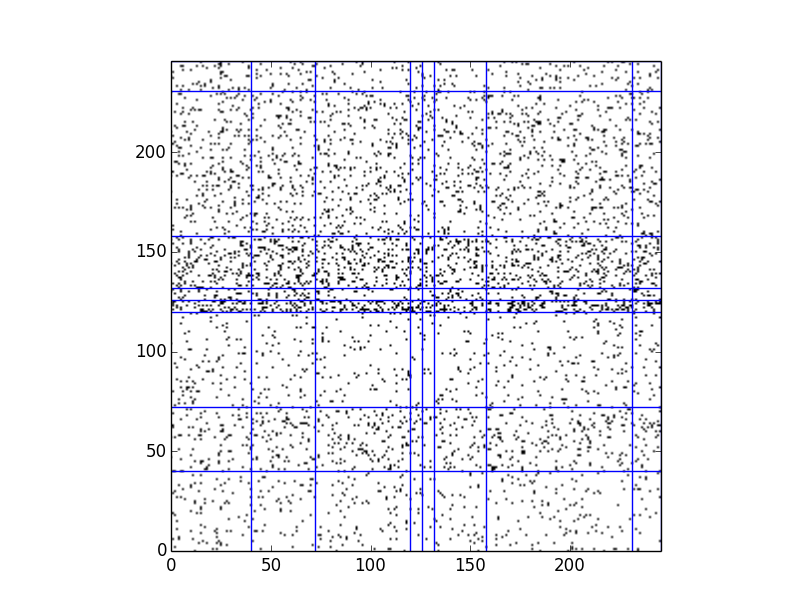
\includegraphics[scale=0.5]{adjacencymatrix.png}}
\newpage

\paragraph{Opportunity}
Graph Models allow us to generate similar graphs from a smaller amount of
parameters.  If we can model connectomes well, then a good model allows us to
generate similar connectomes to perform statistical analysis on similar graphs.
The paper by Pavlovic \cite{pavlovic} used the Erdos Reyni mixture model as an
approximation of the C. Elegans connectome.  Using other graph models to perform
the same analysis will aid future researchers in selecting tools for
connectomics work.

\paragraph{Challenge}
Representing graphs in terms of graph random variables is difficult because
there will always be a loss of information.  Our generated data will be biased
based on the parameters we choose, so it's important that our graph model is
actually useful. Also, choosing appropriate graph metrics for various analysis 
is important and still an active area of research.

\paragraph{Action}
The Random Dot Product Graph Model (RDPG) represents each node by a random
vector, and assigns the probability of edges between nodes to be the dot product
between the two vectors \cite{young}.
Each vector is in $\mathbb{R}^{d}$ with coordinates independently and
identically distributed according to a uniform distribution:
$\frac{1}{\sqrt{d}}\mathbb{U}^{\alpha}$.\\

Here, we use a variant of RDPG, the Random Dot Product Mixture Model, where we
construct blocks in the graph.  Each block $j$ contains vectors whose 
coordinates are independently and indentically distributed according to the
uniform distribution: $\frac{1}{\sqrt{d}}\mathbb{U}^{\alpha_{j}}$.  For n
blocks, we have $n$ parameters which specify the model and determine how
connected blocks will be.\\

We use the node-block clustering from Figure 2 of \cite{pavlovic}, and generate
Random Dot Product Graphs with these blocks.

We applied parameter estimation to the alpha parameters for each block, using a
conjugate gradient method to attempt to converge to a solution.

The graph metric that we are using in optimization is the clustering 
coefficient, which is defined \cite{pavlovic} as the amount of triplets of nodesthat are all connected to each other, divided by the nodes with degree of more 
than 2.  We are trying to minimize the absolute difference between the estimated
graph's clustering coefficient and the true graph's clustering coefficient.

In an attempt to push the algorithm to converge faster, we also added a loss
function.  If the mean degree of nodes in a block is outside of one standard
deviation of the truth's mean node degree for that block, then a penalty is
given to the score by the amount of extra edges (or how many fewer edges there
are) in that block.

Each iteration of the optimization algorithm creates a Random Dot Product Graph
and calculates the graph metric.  An optimal generated graph is then implicitly 
defined as having a near-identical clustering coefficient to the true graph, and
having the mean degree of nodes in every block being within one standard
deviation of the mean degree of nodes in blocks from the true graph.

\paragraph{Resolution}
Shown above is the adjacency matrix that's the result of the parameter
estimation.  It's pretty bad for a few reasons.  First, the way that I organized
the RDP mixture model assigns a random vector to each vertex.  However, when we
block nodes, even if the blocks have their own $\alpha$ parameter, the dot
product between nodes in different blocks will probably be non-zero, and will
generate an edge with a somewhat higher than non-zero probability.

Since the edge probability is pairwise between two vertices, each vertex needs
to have a non-zero vector so that it can have a non-zero degree inside its own
block, but we also want to have very few edges outside of its own local block.

\paragraph{Future Work}
It would be cool to implement the same Random Dot Product Model with blocks that
have orthogonal or near-orthogonal vectors.  This would enable there to be fewer
edges between nodes across blocks.  But this would require the ability to
generate orthogonal random vectors, or random near-orthogonal vectors with a
bounded probability by another parameter.  There may be some way to exploit this
geometrically.

I also wrote code to do spectral embedding but did not get to play around with
that for clustering purposes.  It would be interesting to see to do spectral
embedding for the different blocks in this model, as I've only seen theory
related to spectral embedding for a single RDP graph.

\newpage

\bibliography{main.bib}
\bibliographystyle{plain}


\end{document}  
